\documentclass{standalone}
\usepackage[utf8]{inputenc}
\usepackage[T1]{fontenc}
\usepackage{amsmath,amsfonts,bm}
\usepackage{pgf,tikz}
\usetikzlibrary{arrows}
\begin{document}
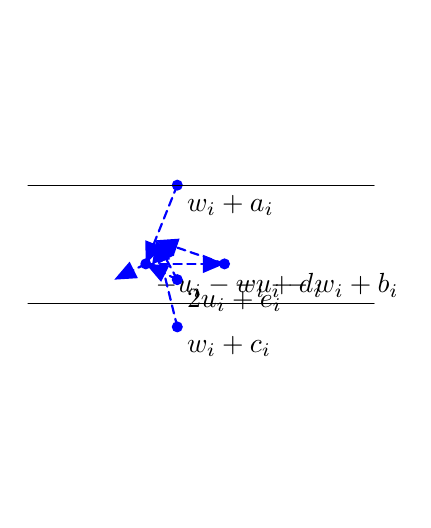
\begin{tikzpicture}[line cap=round,line join=round,>=triangle 45,x=1cm,y=1cm]
    \clip(-2.,-3.) rectangle (2.7608996415757696,3.);
    \fill[color=blue] (-0.1,-0.8) circle (2pt);
    \draw (-0.1,-0.8) node[anchor=north west] {$w_{i}+c_{i}$};
    \fill[color=blue] (-0.1,1.) circle (2pt);
    \draw (-0.1,1.) node[anchor=north west] {$w_{i}+a_{i}$};
    \fill[color=blue] (-0.5,0.) circle (2pt);
    \draw (-0.5,0.) node[anchor=north west] {$-u_{i}-w_{i}+d_{i}$};
    \fill[color=blue] (.5,0.) circle (2pt);
    \draw (.5,0.) node[anchor=north west] {$-u_{i}-w_{i}+b_{i}$};
    \fill[color=blue] (-0.1,-0.2) circle (2pt);
    \draw (-0.1,-0.2) node[anchor=north west] {$2u_{i}+e_{i}$};
    \draw[dash pattern=on 3pt off 2pt,->,line width=0.8pt,color=blue] (-0.1,-0.8)-- (-0.37,0.3);
    \draw[dash pattern=on 3pt off 2pt,->,line width=0.8pt,color=blue] (-0.1,1.)-- (-0.5,0.);
    \draw[dash pattern=on 3pt off 2pt,->,line width=0.8pt,color=blue] (-0.5,0.)-- (-0.9,-0.2);
    \draw[dash pattern=on 3pt off 2pt,->,line width=0.8pt,color=blue] (-0.1,-0.2)-- (-0.37,0.3);
    \draw[dash pattern=on 3pt off 2pt,->,line width=0.8pt,color=blue] (-0.1,-0.2)-- (-0.5,0.);
    \draw[dash pattern=on 3pt off 2pt,->,line width=0.8pt,color=blue] (-0.5,0.)-- (.5,0.);
    \draw[dash pattern=on 3pt off 2pt,->,line width=0.8pt,color=blue] (.5,0.)-- (-0.37,0.3);
    \draw (-0.1,-0.5) parabola[bend pos=0.8] ++(-2.5,0.);
    \draw (-0.1,-0.5) parabola[bend pos=0.8] ++(2.5,0.);
    \draw (-0.1,1.) parabola[bend pos=0.8] ++(-2.5,0.);
    \draw (-0.1,1.) parabola[bend pos=0.8] ++(2.5,0.);
    \end{tikzpicture}
\end{document}